\jxhj{%教学后记
	}
\skrq{%授课日期
	2017年6月6日 4-5节}
\ktmq{%课题名称
	 综合加工}
\jxmb{%教学目标,每行前面要加 \item
	\item 掌握二维图的绘制;
	\item 掌握挖槽加工参数的设置;
	\item 掌握孔加工参数的设置。}
\jxzd{%教学重点,每行前面要加 \item
	\item 二维图的绘制;
	\item 挖槽加工参数的设置。}
\jxnd{%教学难点,每行前面要加 \item
	\item 挖槽加工参数的设置。}
\jjff{%教学方法
	通过讲述、举例、演示法来说明;}

\makeshouye %制作教案首页

%%%%教学内容
\subsection{组织教学}
\begin{enumerate}[\hspace{2em}1、]
	\item 集中学生注意力;
	\item 清查学生人数;
	\item 维持课堂纪律;
\end{enumerate}
\subsection{复习导入及主要内容}
\begin{enumerate}[1、]
	\item 数据线的接法;
	\item 传输过程;
	\item DNC 在线加工。
\end{enumerate}


\subsection{教学内容及过程}

\subsubsection{绘制图形}
如图\ref{二维图}所示:(数铣的第四个课题图)
\begin{figure}[!hbtp]
	\centering	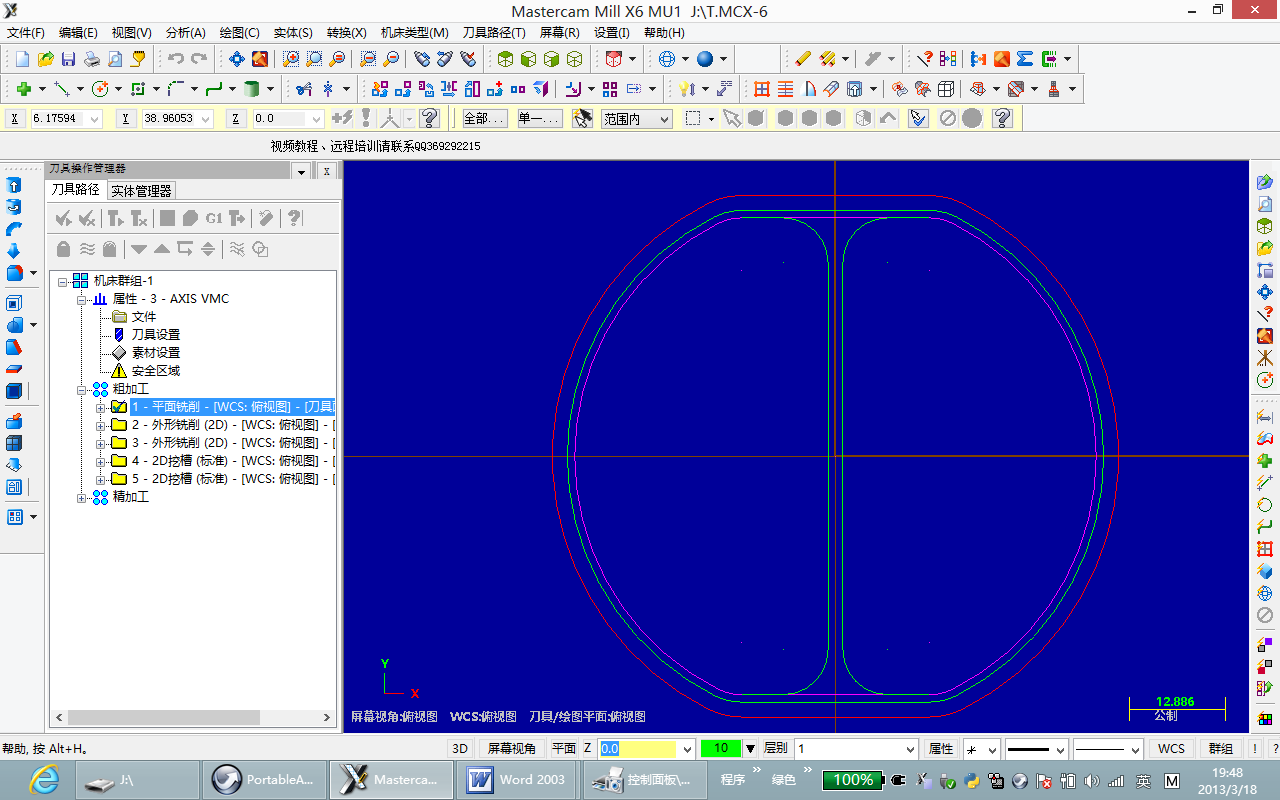
\includegraphics[width=0.95\textwidth]{images/15-1}
	\caption{二维图} \label{二维图}
\end{figure}

绘图工具的使用

1、	圆弧、圆\par
2、	直线、垂直线、水平线的绘制(与cad不一样)\par
3、	图形的修剪与延伸(分割物体、三个物体修剪、两个物体修剪、一个物体修剪、点修剪)延伸与打断\par
4、	倒圆角(修剪与不修剪)\par
5、	单体补正、串联补正(注意补正的方向,最好标注一下)\par
6、	尺寸的标注,(目的是进行检查)\par
7、	图层的操作(显示与关闭、图素图层的更改)\par
\subsubsection{面铣加工}
如图\ref{面铣加工}所示:
\begin{figure}[!hbtp]
	\centering	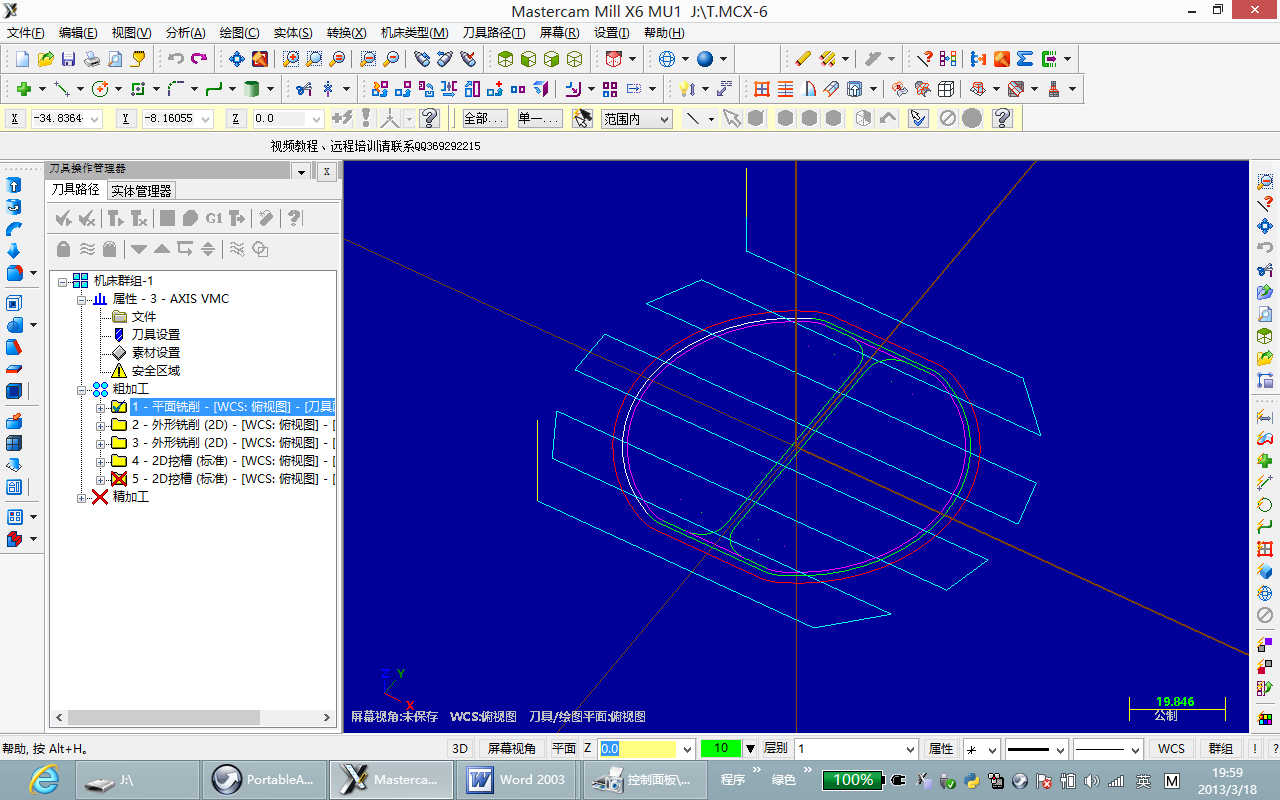
\includegraphics[width=0.95\textwidth]{images/15-2}
	\caption{面铣加工} \label{面铣加工}
\end{figure}

1、	机床的选择(三轴立式铣床)\par
2、	机床参数的设定(刀具、毛坯等)\par
3、	面铣操作\par
图素的选择\par
刀具的选择及参数的设定\par
刀具过滤器、刀具号、补偿号、切削用量等\par
切削参数:\par
加工方向:单向、双向、一刀式、动态\par
对刀位置:刀尖、中心\par
两切削间位移方式:\par
底面预留量:\par
参考高度、安全高度、进给下刀位置、工件表面、深度\par
\subsubsection{外形加工}
如图\ref{外形加工}所示:
\begin{figure}[!hbtp]
	\centering	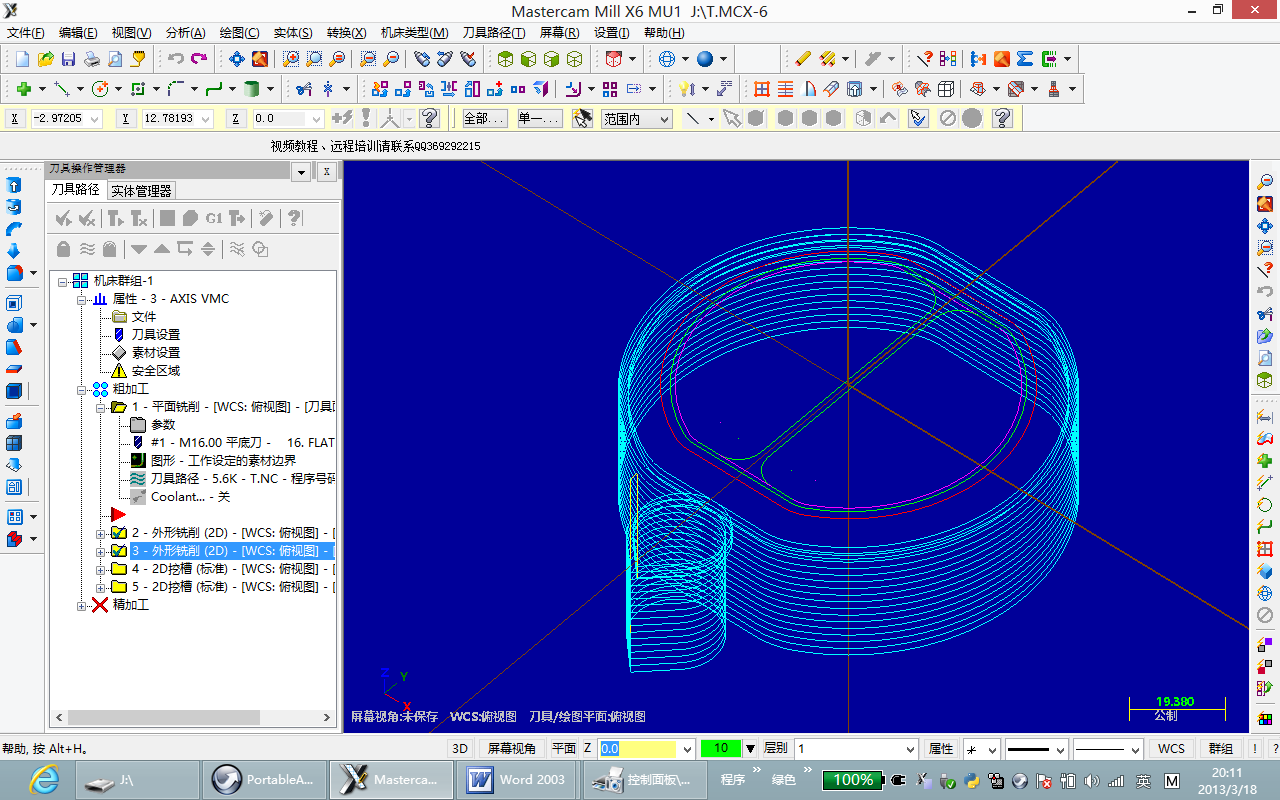
\includegraphics[width=0.95\textwidth]{images/15-3}
	\caption{外形加工} \label{外形加工}
\end{figure}
1、图素的选择\par
2刀具的选择及参数的设定\par
刀具过滤器、刀具号、补偿号、切削用量等\par
3、切削参数:\par
补正方式\par
补正方向\par
刀具在转角处走圆角\par
外形切削方式\par
壁边预留量\par
底边预留量\par
4、参考高度、安全高度、进给下刀位置、工件表面、深度\par
5、Z向分层加工\par
6、XY向分层加工\par
7、切入切出的设定\par
8、切入切出点的设定\par
9、加工方向补偿方向的改变。\par
\subsubsection{刀路的检查与模拟}
1、	二维图形模拟\par
刀具的显示\par
着色显示\par
Z向坐标显示\par
2、	实体验证\par
如图\ref{实体验证}所示:
\begin{figure}[!hbtp]
	\centering	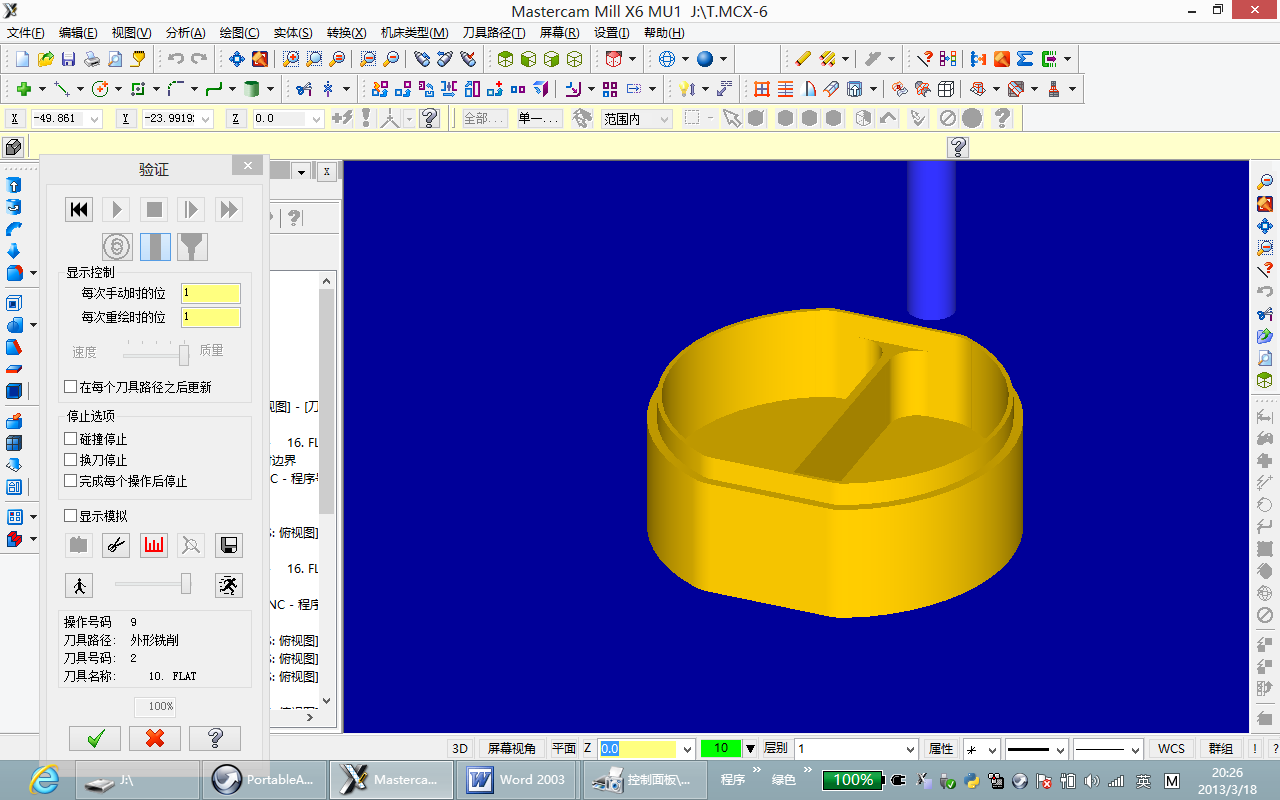
\includegraphics[width=0.95\textwidth]{images/15-4}
	\caption{实体验证} \label{实体验证}
\end{figure}
\subsubsection{应用、完成零件加工、后处理、生成加工程序}
如图\ref{完成零件}所示:
\begin{figure}[!hbtp]
	\centering	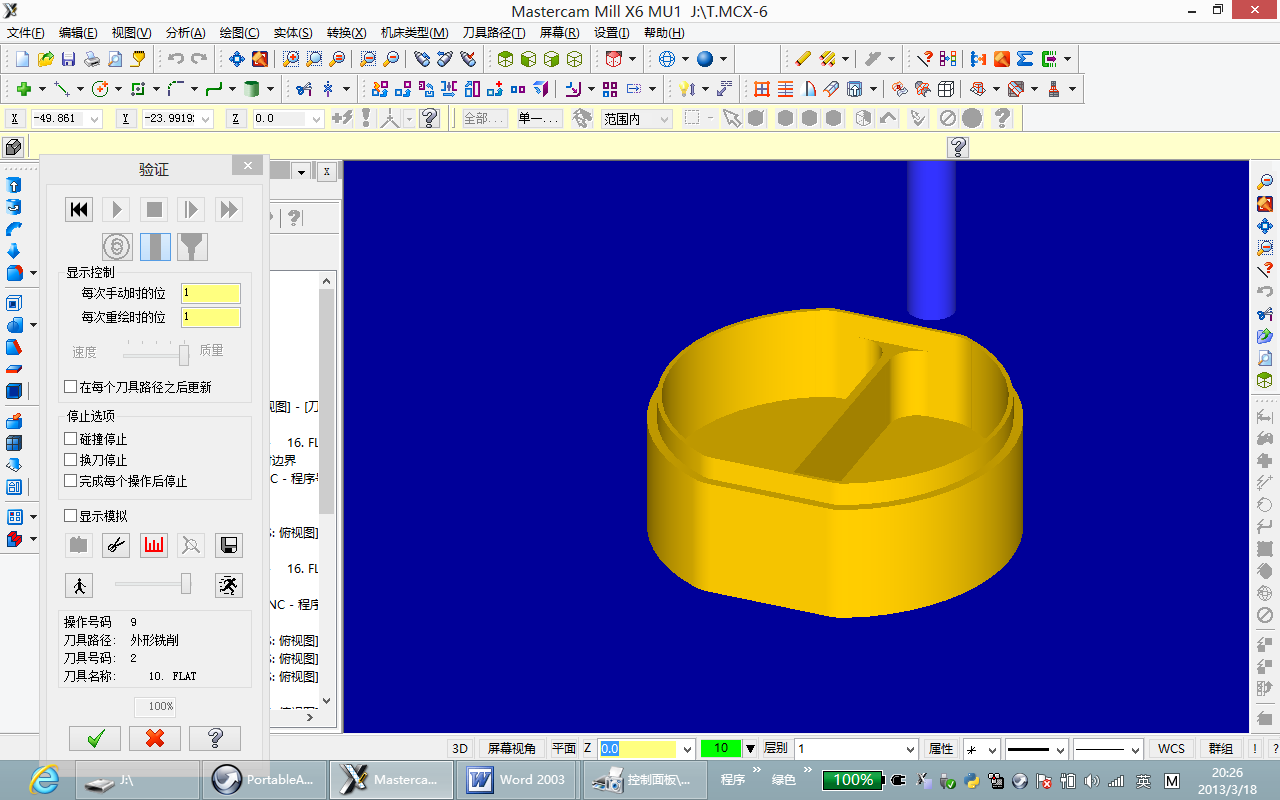
\includegraphics[width=0.95\textwidth]{images/15-4}
	\caption{完成零件} \label{完成零件}
\end{figure}	
\subsubsection{其他图形的练习}

自己练习










\subsection{课堂小结}
\begin{enumerate}[1、]
	\item 绘制图形;
	\item 面铣加工;
	\item 外形加工。
\end{enumerate}

\vfill
\subsection{布置作业}
\begin{enumerate}[1、]
	\item 自选图,完成简单零件的自动加工。
\end{enumerate}
\vfill